\section{Retrieval design and experiments (Q3)}
\subsection{Retrieval problems and design}
Scientific questions may use different wording from the passages that answer them, while exact dataset and model names remain important. We combine lexical and dense retrieval to address these complementary matching needs. Reranking tests whether joint query--passage scoring improves candidate ordering, while chunk-size and retrieval-depth experiments examine the trade-off between evidence coverage and the amount of text supplied.

\textbf{Complementary retrieval.} BM25 \citep{robertson2009bm25} uses term matching with term-frequency saturation and passage-length normalization. Our implementation applies case folding and Unicode word-token extraction, with $k_1=1.5$ and $b=0.75$. Dense retrieval uses \texttt{BAAI/bge-small-en-v1.5} \citep{baai2023bgesmallv15} to encode queries and passages, ranking L2-normalized vectors through per-paper FAISS exact inner-product search. A search instruction is prepended to queries only. Evaluation ranks passages within the selected paper.

\textbf{Hybrid fusion.} Each retriever returns up to 20 candidates. We deduplicate by passage ID and combine rankings using reciprocal rank fusion \citep{cormack2009rrf}:
\begin{equation}
\operatorname{RRF}(p)=\sum_{s:p\in L_s}\frac{1}{60+\operatorname{rank}_s(p)}.
\end{equation}
Ranks start at one; a passage absent from a list contributes nothing for that source. Fusion combines lexical and vector rankings without assuming their scores have comparable scales.

\textbf{Reranking and input limits.} We tested \texttt{BAAI/bge-reranker-base}, a cross-encoder that jointly scores each query and passage, on the fused candidate union. The dense encoder limits each encoded input to 512 tokens; the reranker applies a 512-token limit to the combined query--passage input. In the reported corpus, 14.3\% of passages exceed the dense encoder's limit; BM25 reads their full text. This may affect which evidence is represented, but its effect on retrieval quality was not isolated. Generation-side clipping is discussed in Q4.2.

\hyperref[fig:hybrid]{Figure~\ref*{fig:hybrid}} shows the retrieval branches, fusion, evidence pool and retry path.
\begin{figure}[htbp]\centering
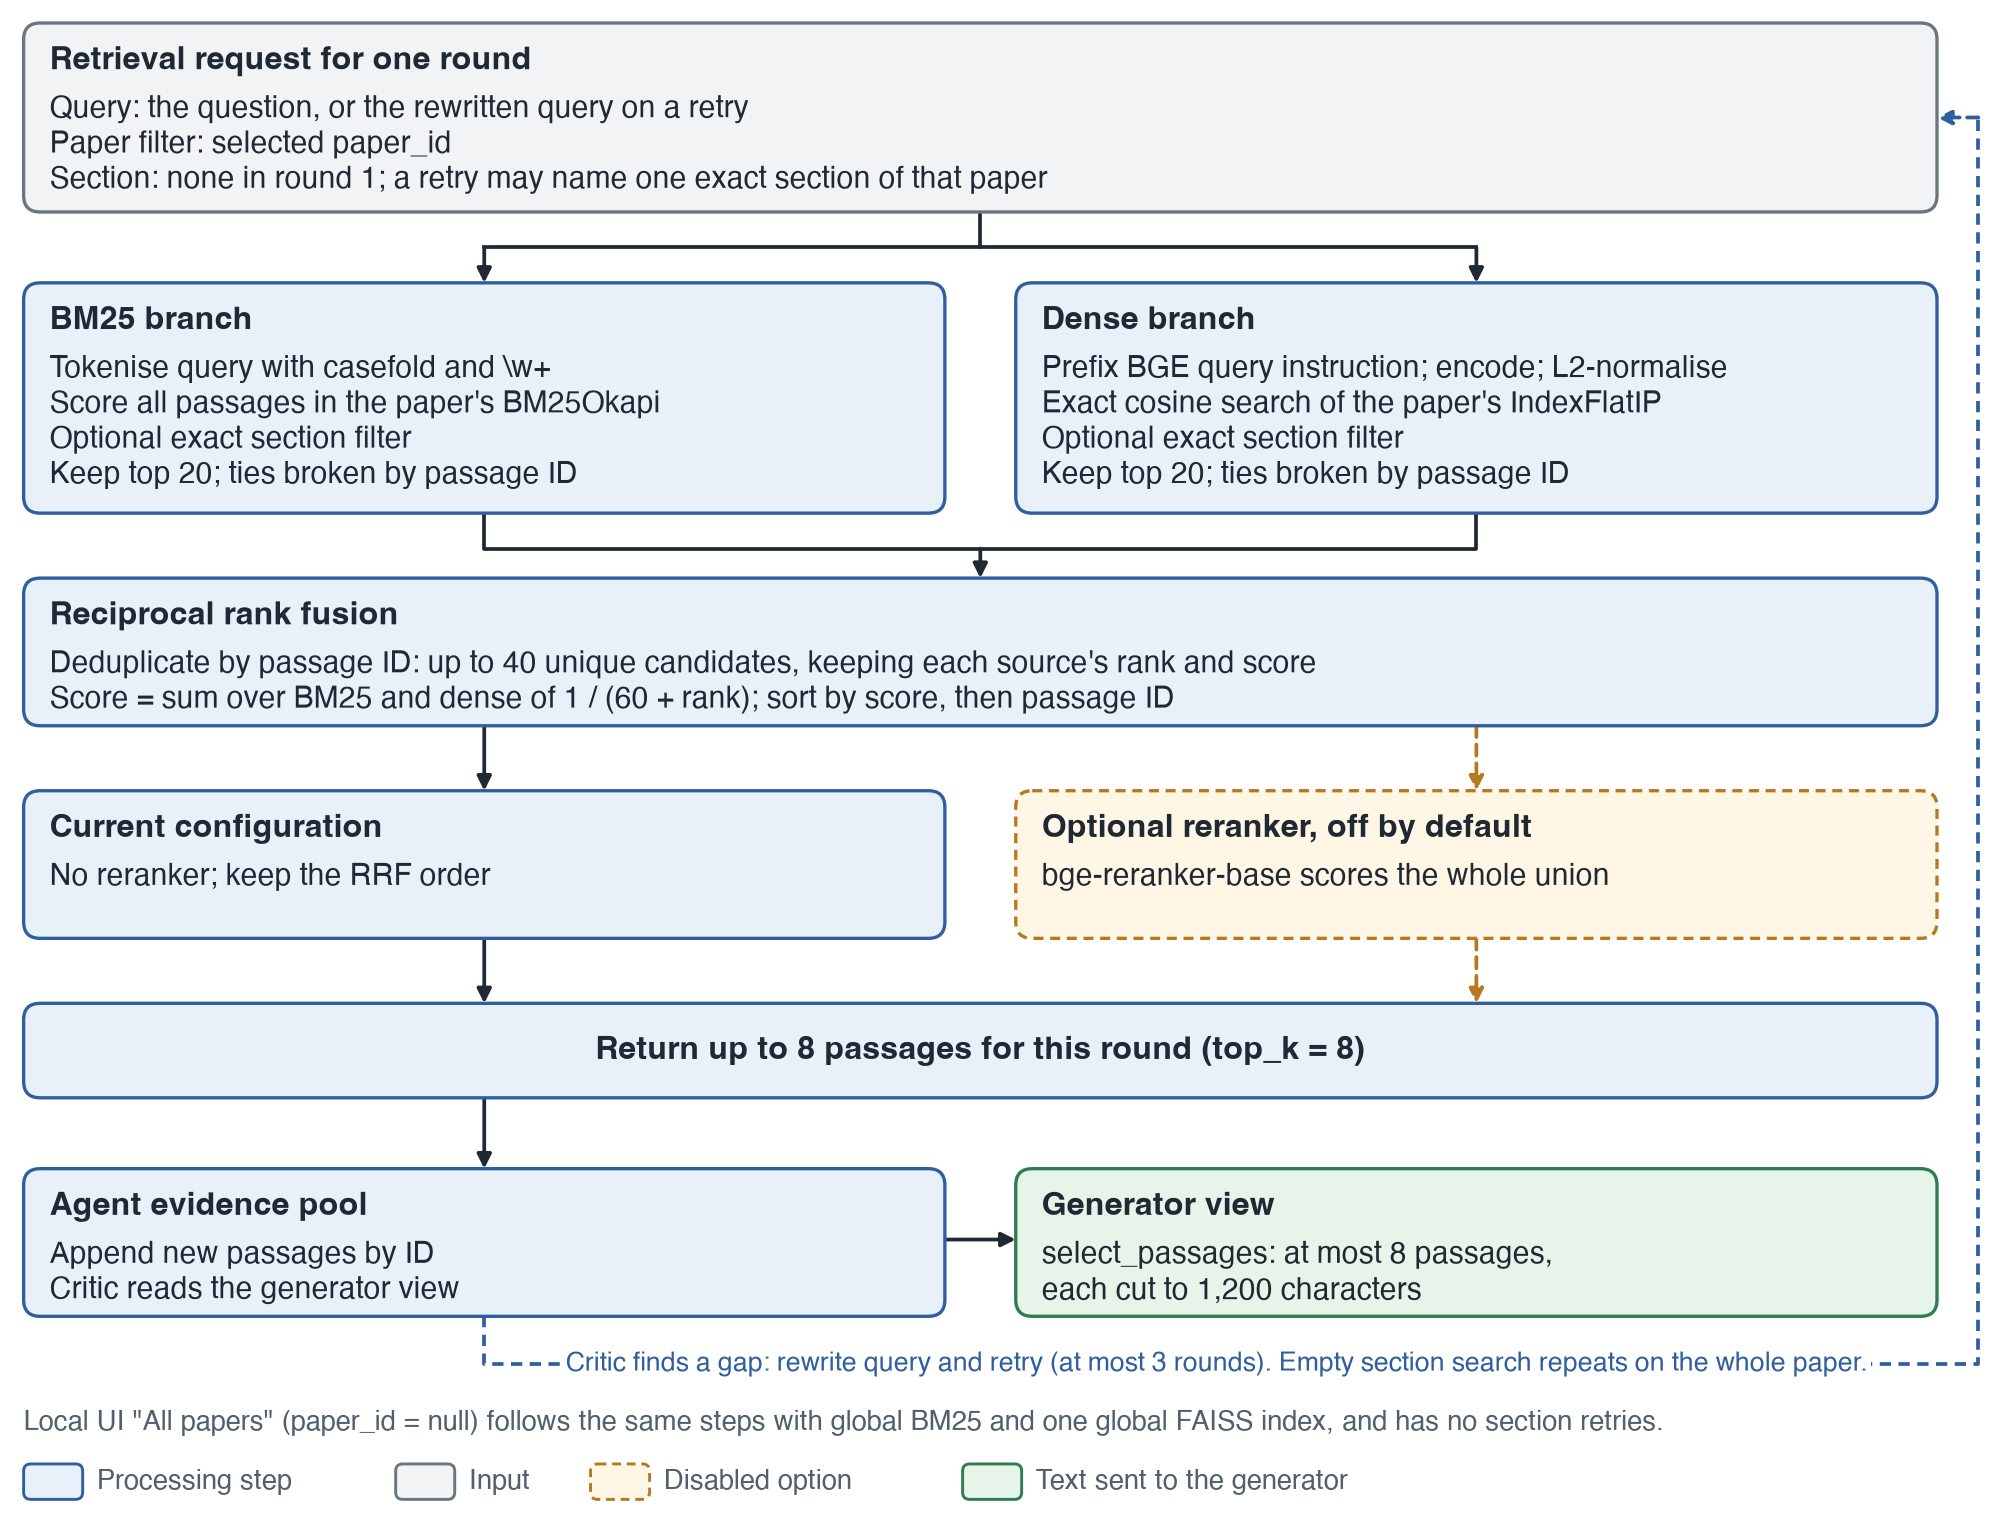
\includegraphics[width=\linewidth,height=0.78\textheight,keepaspectratio]{images/online-hybrid-retrieval.png}
\caption{Online hybrid retrieval and the bounded retry loop. The current configuration returns up to eight RRF passages per round without reranking; the optional reranker is shown as a disabled comparison. The critic and generator use the same clipped evidence view. This top-eight agent setting is separate from the reported retrieval evaluation at $K=5$.}\label{fig:hybrid}
\end{figure}


\subsection{Evaluation setup and rank-aware results}
% Generated from results/p6/retrieval-draft-v3/summary.json
\begin{table}[htbp]\centering
\caption{Development retrieval on draft labels. Recall and nDCG are relative to the judged pool.}\label{tab:retrieval}
\begin{tabular}{lrrrr}\toprule
Method & P@5 & Pool R@5 & MRR@5 & Pool nDCG@5\\\midrule
BM25 & 0.482 & 0.607 & 0.730 & 0.636\\
Dense & 0.527 & 0.698 & 0.799 & 0.719\\
Hybrid RRF & 0.539 & 0.714 & 0.804 & 0.731\\
RRF + reranker & 0.509 & 0.659 & 0.718 & 0.663\\\bottomrule\end{tabular}\end{table}

The frozen ranking pool contains four methods for 200 questions, evaluated against the accepted binary question--passage label file. \hyperref[tab:retrieval]{Table~\ref*{tab:retrieval}} reports scores from the accepted-label run. Precision@5 measures relevant results among the five returned slots; MRR@5 rewards an early first relevant passage. Pool-relative recall measures recovery of the relevant passages that were judged, not every relevant passage in the paper. Binary nDCG discounts relevant passages by rank and normalizes against the ideal ranking within the judged pool.

The judged pool is the deduplicated union of the four methods' saved top-five results, comprising 1,853 question--passage pairs. All scored top-five results are judged. Scores are macro-averaged with equal weight per question: precision and MRR use 200 questions, while pool recall and nDCG exclude one question with no positive labels, leaving 199. The pool is not exhaustive: relevance outside it remains unknown, so scoring other methods or deeper cutoffs may require additional judgments.

RRF achieves the highest mean scores in \hyperref[tab:retrieval]{Table~\ref*{tab:retrieval}}. The paired comparisons below assess whether its differences from the other methods are consistent across questions. Annotation provenance and its limitations are described in Section~\ref{sec:annotation}.

\subsubsection{Fusion and reranking comparisons at \texorpdfstring{$K=5$}{K=5}}
\begin{table}[htbp]\centering\small
\caption{Fusion and reranking comparisons at $K=5$. Differences are the first method minus the second. Intervals use 1,000 paper-cluster bootstrap resamples, seed 42, over 174 papers.}\label{tab:p2-paired}
\begin{tabularx}{\linewidth}{YYrrl}\toprule
Comparison & Metric & Difference & $n$ & 95\% interval\\\midrule
RRF -- BM25 & Precision & +0.0570 & 200 & [+0.0354, +0.0788]\\
RRF -- BM25 & Pool recall & +0.1070 & 199 & [+0.0663, +0.1471]\\
RRF -- BM25 & MRR & +0.0747 & 200 & [+0.0398, +0.1112]\\
RRF -- BM25 & Pool nDCG & +0.0958 & 199 & [+0.0640, +0.1273]\\
RRF -- Dense & Precision & +0.0120 & 200 & [-0.0063, +0.0318]\\
RRF -- Dense & Pool recall & +0.0161 & 199 & [-0.0139, +0.0462]\\
RRF -- Dense & MRR & +0.0052 & 200 & [-0.0330, +0.0434]\\
RRF -- Dense & Pool nDCG & +0.0125 & 199 & [-0.0154, +0.0409]\\
RRF+BGE -- RRF & Precision & -0.0300 & 200 & [-0.0555, -0.0051]\\
RRF+BGE -- RRF & Pool recall & -0.0550 & 199 & [-0.1037, -0.0098]\\
RRF+BGE -- RRF & MRR & -0.0868 & 200 & [-0.1377, -0.0350]\\
RRF+BGE -- RRF & Pool nDCG & -0.0682 & 199 & [-0.1123, -0.0256]\\
\bottomrule\end{tabularx}\end{table}

\hyperref[tab:p2-paired]{Table~\ref*{tab:p2-paired}} uses paired question scores and 1,000 paper-cluster bootstrap resamples (seed 42). Each resample draws 174 papers with replacement, retains their valid question pairs, and computes the question-weighted mean difference; endpoints are the 2.5th and 97.5th percentiles. Precision/MRR use 200 questions, and pool recall/nDCG use 199. RRF improves on BM25 across all four metrics, with all intervals above zero. RRF has only small gains over Dense; intervals that include zero do not establish a reliable improvement. The tested reranker produces lower aggregate scores than RRF across all four metrics; its unadjusted paired intervals are below zero. These are 12 exploratory comparisons without multiple-comparison correction, and the intervals do not account for annotation bias. The results therefore describe this evaluated pool rather than a general ordering of retrieval methods.

The four-method comparison is evaluated at $K=5$. The agent's top-eight RRF configuration was selected separately using development evidence-recall results, discussed below.

\subsubsection{Paired BM25--Dense comparison at \texorpdfstring{$K=5$}{K=5}}
% Means: results/p2-final-retrieval-handoff/scored/retrieval.csv.
% Paired differences and intervals: results/p1-bm25-vs-dense-verification-20261105/comparison/ablation.csv.
% Differences use the unrounded per-question scores, not rounded table means.
\begin{table}[htbp]\centering\small
\caption{BM25 versus Dense at $K=5$ on the accepted relevance labels. Differences are Dense minus BM25. Percentile intervals use 1,000 paper-cluster bootstrap resamples, seed 42; all rows cover 174 papers. $n$ denotes questions.}\label{tab:bm25-dense-paired}
\begin{tabularx}{\linewidth}{Yrrrrl}\toprule
Metric & BM25 & Dense & Difference & $n$ & 95\% interval\\\midrule
Precision & 0.4820 & 0.5270 & $+0.0450$ & 200 & [0.0171, 0.0728]\\
Pool recall & 0.6067 & 0.6976 & $+0.0909$ & 199 & [0.0419, 0.1421]\\
MRR & 0.7296 & 0.7992 & $+0.0696$ & 200 & [0.0168, 0.1222]\\
Pool nDCG & 0.6355 & 0.7188 & $+0.0833$ & 199 & [0.0366, 0.1314]\\\bottomrule
\end{tabularx}
\end{table}

Dense has higher mean scores than BM25 on all four metrics in this judged pool. The Precision@5 gain of 4.50 percentage points corresponds to an average of 0.225 additional passages labelled relevant per question among the five returned slots. Pool recall improves by approximately 9.09 percentage points. These results favour Dense over BM25 as a single-retriever quality baseline for this fixed evaluation at $K=5$; downstream answer quality is not measured here.

\hyperref[tab:bm25-dense-paired]{Table~\ref*{tab:bm25-dense-paired}} uses the same paper-cluster bootstrap procedure and metric denominators as the fusion comparisons. All four intervals are above zero. These findings are conditional on the evaluated questions and accepted labels; pool-relative recall is not exhaustive paper-level recall.

\subsection{Illustrative query comparisons}
\paragraph{Complementary BM25 and Dense results.}
The examples below illustrate contrasting outcomes within the evaluated pool. They use the accepted relevance labels and were selected to explain ranking behavior, not to estimate its frequency or establish generated-answer correctness.

For ``Which commonsense knowledge base are they using?'' (paper \texttt{1709.05453}; \citep{young2017dialog}), Dense retrieves both passages labelled relevant at ranks one and five; BM25 retrieves neither in its saved top five. The rank-five passage states, ``In our experiment, ConceptNet is used as the commonsense knowledge base.'' Dense's precision is 0.4 and pool recall is 1.0, compared with zero for BM25 on both metrics. This illustrates the evidence retrieved by Dense at the evaluated cutoff; the cause of the ranking difference was not isolated.
% Question 042800c3336ed5f4826203616a39747c61382ba6. Exact passage IDs: review-checks/p1-evidence.md.

For ``What baselines do they propose?'' (paper \texttt{2003.12660}; \citep{ahia2020pidgin}), BM25 retrieves relevant passages at ranks three and five describing supervised and unsupervised translation baselines, tokenization variants and their architecture. The rank-five passage states, ``All baseline models were trained using the Transformer architecture''. The rank-five hit has a BM25 score of zero and is ordered by passage ID among ties, so its inclusion should not be interpreted as a strong lexical match. Dense retrieves no passage labelled relevant in its saved top five. BM25's precision is 0.4 and pool recall is 0.5, compared with zero for Dense on both metrics. Dense's fourth and fifth passages mention supervised and unsupervised models, but are labelled non-relevant in the accepted labels. The example illustrates query-specific complementarity under the recorded judgments: Dense's higher aggregate scores do not mean that it retrieves more relevant evidence for every question.
% Question dd81f58c782169886235c48b8f9a08e0954dd3ae. Exact passage IDs: review-checks/p1-evidence.md.

\paragraph{Contrasting effects of reranking.}
For ``How effective is their NCEL approach overall?'' (paper \texttt{1811.08603}; \citep{cao2018ncel}), RRF returns the three pool passages labelled relevant at ranks one, three and four. The rank-one passage describes NCEL outperforming baselines on both easy and hard entity-linking datasets; the rank-three passage gives a concrete disambiguation example, and rank four summarizes evaluation across five benchmarks. BGE retains only the last of these at rank four in its top five. RRF precision/pool recall are 0.6/1.0, versus 0.2/0.3333 after reranking. The relevant evidence excluded from BGE's top five is known from the saved outputs; its exact lower ranks are not available. This example illustrates a change in the top-five evidence set; it does not identify the cause.
% Question 114934e1a1e818630ff33ac5c4cd4be6c6f75bb2; passage IDs: review-checks/p2-evidence.md.


The rank-three NCEL passage is a debatable relevance judgment for overall effectiveness. Even excluding that passage from both methods, RRF retains two accepted relevant passages versus one with BGE. The published scores retain the accepted gold unchanged.

\paragraph{A contrasting reranking improvement.}
For ``what are the state of the art models?'' (paper \texttt{1803.09000}), reranking increases Precision@5 from 0.2 to 0.4 under the accepted labels, although MRR@5 falls from 0.5 to 0.3333 because its first relevant passage moves from rank two to rank three. The precision gain depends on one passage whose two annotators disagreed and whose final label was resolved during review. This illustrates a query-specific precision gain alongside a lower reciprocal rank, despite the reranker's lower aggregate scores.
% Question d7799d26fe39302c4aff5b530aa691e8653fffe8; source: pinned P2 scores.jsonl, rankings and accepted labels.


\subsection{Chunk size and retrieval depth}
We compared BM25 chunk sizes through a coarse-to-fine search, holding overlap at 40 words and retrieval within the question's paper. Initial experiments on 50 questions narrowed the candidates to 325, 365 and 375 words. A final comparison used 200 additional questions fixed before retrieval. All 250 selection questions were excluded from the final relevance evaluation.

The comparison uses questions whose supporting evidence can be fully and unambiguously located in the paper text. An evidence hit means that the retrieved text jointly covers at least one complete annotated evidence paragraph; complete evidence means covering every supporting paragraph for at least one reference answer. We compare coverage under fixed reading budgets of 500, 1,000 and 2,000 words, counting overlapping text each time it appears and cutting the final passage to fit. Top-five coverage is supplementary because larger chunks also supply more text.

On the 200 additional questions, 365-word chunks give slightly higher top-five coverage than 375-word chunks: 147 versus 145 evidence hits and 125 versus 123 complete-evidence successes. They also require slightly less reading (1,247 versus 1,262 words on average). However, under the primary 1,000-word budget, 375 words covers complete evidence for 108 questions versus 106 for 365; at 500 words, 325 performs best with 75 successes. We chose 365/40 as a compromise between coverage and reading volume. Overlap was held fixed rather than tuned.

A separate agent development slice contains 40 questions, of which 32 have mapped evidence. Static RRF evidence recall rises from 0.740 at top five to 0.885 at top eight and 0.974 at top ten. Complete evidence is recovered for 22, 26 and 30 of the 32 questions, respectively. These are mapped-evidence metrics, distinct from relevance-pool recall in \hyperref[tab:retrieval]{Table~\ref*{tab:retrieval}}. Top eight matches the generator's passage-count limit; top ten is a retrieval diagnostic and exceeds that limit.
The frozen downstream evaluation supplies a separate depth analysis on 200 questions with 347 mapped gold passages, using one saved ranking per question. Plain retrieval recovers 0.723 of the mapped evidence at five passages, 0.858 at eight, 0.897 at ten and 0.953 at fifteen (\hyperref[tab:depth]{Table~\ref*{tab:depth}}). The ordering matches the development slice, but the curve is flatter: ten passages recover 0.897 here against 0.974 on the slice, showing that the size of the depth gain varies between question sets. The eight-passage setting was chosen on development evidence and was not changed afterwards. Because the agent developer labelled 40 of these questions for annotation before the freeze, we also report the remaining 160; both subsets show increasing recall with depth. Mapped-evidence recall differs from the pool-relative recall of \hyperref[tab:retrieval]{Table~\ref*{tab:retrieval}}.
\begin{table}[htbp]\centering\small
\caption{Mean mapped gold recall of plain retrieval by depth (no critic, no retry); complete evidence in brackets. Held-out depths come from one 15-passage ranking. ``160 not annotated'': held-out questions the agent developer did not annotate.}\label{tab:depth}\vspace{1.5mm}
\begin{tabularx}{\linewidth}{>{\hsize=1.8\hsize\linewidth=\hsize}Y>{\hsize=0.84\hsize\linewidth=\hsize}Y>{\hsize=0.84\hsize\linewidth=\hsize}Y>{\hsize=0.84\hsize\linewidth=\hsize}Y>{\hsize=0.84\hsize\linewidth=\hsize}Y>{\hsize=0.84\hsize\linewidth=\hsize}Y}\toprule
Questions & Top 3 & Top 5 & Top 8 & Top 10 & Top 15\\\midrule
Development slice (32) & 0.599 (17) & 0.740 (22) & 0.885 (26) & 0.974 (30) & 0.974 (30)\\
Held-out, all 200 & 0.569 (84) & 0.723 (117) & 0.858 (154) & 0.897 (166) & 0.953 (183)\\
Held-out, 160 not annotated & 0.585 (69) & 0.749 (98) & 0.881 (127) & 0.907 (134) & 0.959 (148)\\\bottomrule\end{tabularx}
\end{table}
\begin{figure}[htbp]\centering
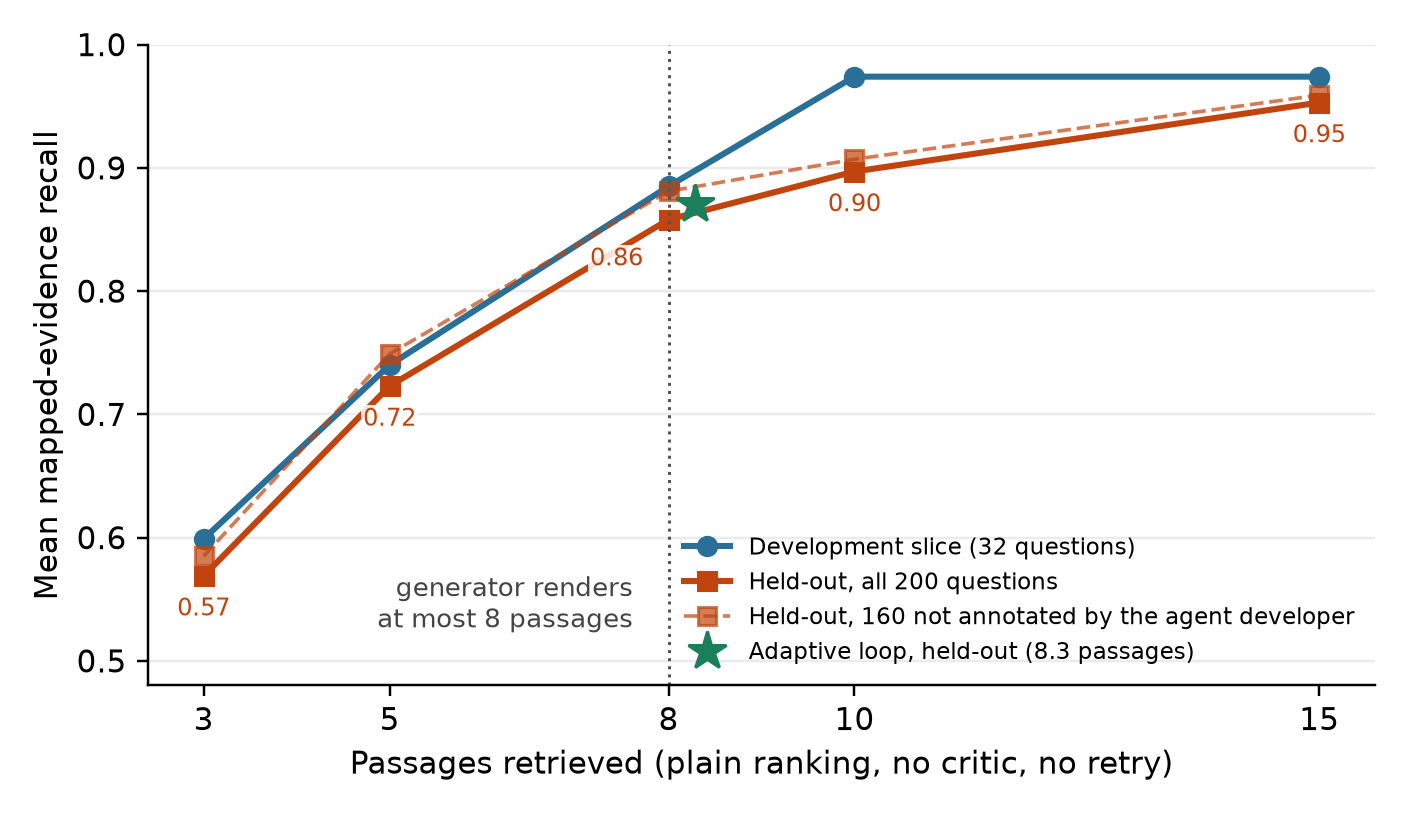
\includegraphics[width=0.92\linewidth]{images/recall-by-depth.png}
\caption{Mean mapped-evidence recall of plain retrieval by depth (the values of \hyperref[tab:depth]{Table~\ref*{tab:depth}}). The development slice reaches 0.974 at ten passages, the held-out curve is flatter (0.897 at ten), and the adaptive result on the held-out questions (star) is close to plain retrieval at a comparable passage budget. The generator renders at most eight passages.}\label{fig:depth}
\end{figure}
\paragraph{Evidence recovered by increasing depth.} For ``Where did they get the data for this project?'' (development paper \texttt{1805.11535}; reference answer: Twitter), the passage labelled as evidence is ranked seventh. It states, ``Our dataset is constructed via distant supervision from Twitter.'' Top-five retrieval excludes it, whereas top eight includes it. The 599-character passage fits within the generator's context limit. This is a concrete improvement in evidence access; the generated answer cites a different passage, so the example does not establish an answer-grounding improvement.

\subsection{Resulting retrieval configuration}
RRF combines complementary rankings and improves on BM25 across the evaluated metrics, while its gains over Dense are small and uncertain. The tested reranker offers no aggregate benefit on this pool, although individual queries show gains. We therefore retain RRF without reranking. The 365/40 chunk configuration balances evidence coverage and reading volume; top eight was selected using development evidence and matches the generator's passage limit. Deeper rankings measure retrieval coverage beyond the rendered context, rather than evidence actually used by generation. The effects of adaptive query rewriting and its downstream ablations are reported in Q5.

% Assessment retained internally; 5/5 review boxes are hidden.
% \begin{review}{Q3: AI-suggested five-star implementation self-check}
\draftreview{P2}{P1, P3, P4, P6}{P2 leads fusion/reranking results; P1 checks sparse/dense comparisons; P3 checks chunking and gold; P4 checks depth results; P6 cross-checks scoring and tables.}
\colorbox{yellow!45}{\strut\textbf{DONE FOR DRAFT --- P1}}\par
Approved by Junlin Yin on 6 November 2026 for the BM25/Dense methods, paired comparison and two contrasting examples. Other owners' reviews remain pending.\par\smallskip
\textbf{P2 technical checks complete; owner approval pending.}\par Numerical comparisons and examples checked against saved outputs; Vishakha must confirm final wording before replacing this with an owner sign-off.\par\smallskip
\aistars{3}\quad\textbf{Provisional AI assessment: 3/5 stars. Target: 5/5 --- strong implementation.} This is an editorial assessment, not a course grade. Sparse, dense, hybrid and reranked comparisons are implemented, and the negative reranking result is reported clearly. Accepted-label results and the independently reproduced BM25--Dense paired intervals are now included. P1's contrasting examples have been confirmed by Junlin Yin; P2 paired comparisons and a traceable reranking failure example are now incorporated; member sign-off on final wording remains pending. Confirm evaluation roles and the fusion/depth example, preserve the different denominators, and distinguish pool-relative relevance recall from mapped-evidence recall. Confirm that explanations for reranker failure remain hypotheses unless tested. This P1 approval does not complete owner sign-off for the whole Q3 section.
\end{review}

